\documentclass[11pt,a4paper]{article}

\usepackage[margin=2.2cm]{geometry}
\usepackage{amsmath,amssymb,amsthm}
\usepackage{booktabs}
\usepackage{array}
\usepackage{tabularx}
\usepackage[shortlabels]{enumitem}
\usepackage{xcolor}
\usepackage{tikz}
\usepackage{fancyhdr}
\usepackage{setspace}
\usepackage{microtype}
\usepackage{titlesec}
\usepackage{hyperref}
\usepackage{listings}
\usepackage[skins,breakable]{tcolorbox}

\usetikzlibrary{positioning,arrows.meta,calc,fit,shapes.geometric,matrix,decorations.pathreplacing}

\definecolor{ink}{HTML}{222222}
\definecolor{rulegray}{HTML}{444444}
\definecolor{boxline}{HTML}{666666}
\definecolor{boxfill}{HTML}{F4F4F4}
\definecolor{boxtitle}{HTML}{E8E8E8}
\definecolor{g1}{HTML}{D0D0D0}
\definecolor{g2}{HTML}{9A9A9A}
\definecolor{g3}{HTML}{5A5A5A}

\hypersetup{
  colorlinks=true,
  linkcolor=black,
  urlcolor=black,
  pdftitle={MTL 458 Lecture 21: Persistence: I/O Devices},
  pdfauthor={Minati De, IIT Delhi}
}

\setstretch{1.12}
\raggedbottom
\setlist[itemize]{leftmargin=1.3em,itemsep=0.28em,topsep=0.35em}
\setlist[enumerate]{leftmargin=1.5em,itemsep=0.35em,topsep=0.4em}

\titleformat{\section}
  {\Large\bfseries\color{ink}}{\thesection.}{0.6em}{}
  [{\color{rulegray}\titlerule[0.5pt]}]
\titleformat{\subsection}
  {\large\bfseries\color{ink}}{\thesubsection}{0.55em}{}
\titleformat{\subsubsection}
  {\normalsize\bfseries\color{ink}}{\thesubsubsection}{0.5em}{}

\titlespacing*{\section}{0pt}{1.35em}{0.7em}
\titlespacing*{\subsection}{0pt}{1.05em}{0.45em}

\pagestyle{fancy}
\fancyhf{}
\renewcommand{\headrulewidth}{0.4pt}
\renewcommand{\footrulewidth}{0.3pt}
\fancyhead[L]{\small\color{ink}MTL 458 \textbullet\ Operating Systems}
\fancyhead[R]{\small\color{ink}Lecture 21: Persistence: I/O Devices}
\fancyfoot[C]{\small\thepage}
\setlength{\headheight}{14pt}

% ---------------------------------------------------------------------------
% Boxes
% ---------------------------------------------------------------------------
\tcbset{
  commonbox/.style={
    colback=boxfill, colframe=boxline, boxrule=0.5pt,
    left=6pt, right=6pt, top=5pt, bottom=5pt,
    fonttitle=\bfseries, coltitle=black, colbacktitle=boxtitle,
    enhanced, sharp corners=south, breakable
  }
}
\newtcolorbox{keybox}[1][]{commonbox, title={#1}}
\newtcolorbox{quizbox}[1][]{commonbox, title={#1}}
\newtcolorbox{solbox}[1][]{commonbox, title={#1}}
\newtcolorbox{warnbox}[1][]{commonbox, title={#1}}
\newtcolorbox{defbox}[1][]{commonbox, title={#1}}

\lstset{
  language=C,
  basicstyle=\ttfamily\small,
  keywordstyle=\bfseries,
  commentstyle=\itshape\color{g3},
  numbers=left, numberstyle=\scriptsize\color{g2}, numbersep=6pt,
  frame=single, rulecolor=\color{boxline},
  backgroundcolor=\color{boxfill},
  xleftmargin=1.6em, framexleftmargin=1.4em,
  columns=fullflexible, keepspaces=true,
  showstringspaces=false, breaklines=true,
  aboveskip=0.6em, belowskip=0.6em
}

\newcommand{\strike}[1]{\tikz[baseline=(t.base)]{\node[inner sep=0pt] (t) {#1}; \draw[thick] (t.west) -- (t.east);}}

% Start a new page unless at least #1 of vertical space remains
\makeatletter
\newcommand{\keepspace}[1]{\par\penalty-100\begingroup
  \setlength{\dimen@}{#1}\dimen@ii\pagegoal\advance\dimen@ii-\pagetotal
  \ifdim\dimen@>\dimen@ii\ifdim\dimen@ii>\z@\vfil\fi\break\fi\endgroup}
\makeatother

% ---------------------------------------------------------------------------
% Timeline segments: \seg{y}{x1}{x2}{label}{fill}{text colour}
% CPU row at y = 0.75, Disk row at y = 0
% ---------------------------------------------------------------------------
\newcommand{\seg}[6]{%
  \draw[fill=#5] (#2,#1) rectangle (#3,{#1+0.45});
  \node[font=\small\bfseries, text=#6] at ({(#2+#3)/2},{#1+0.225}) {#4};}
\newcommand{\rows}[1]{%
  \node[anchor=east, font=\small\bfseries] at (-0.15,0.975) {CPU:};
  \node[anchor=east, font=\small\bfseries] at (-0.15,0.225) {Disk:};
  \draw[-{Latex}, g3] (0,-0.35) -- (#1,-0.35) node[right, font=\scriptsize] {time};}
% process colours
\newcommand{\A}{g3}\newcommand{\B}{g1}\newcommand{\C}{black!85}

% ---------------------------------------------------------------------------
% Top view of a platter with 3 tracks x 8 sectors (0-7 inner, 8-15 middle,
% 16-23 outer), numbered clockwise from 12 o'clock.
% \platter{rotation (deg, ccw)}{head radius}{head angle}{show head: 1/0}
% ---------------------------------------------------------------------------
\newcommand{\platter}[4]{%
\begin{tikzpicture}[scale=0.78]
  \fill[g2] (0,0) circle (2.05);
  \foreach \r in {0.95,1.5,2.05} \draw[white, line width=0.8pt] (0,0) circle (\r);
  \foreach \k in {0,...,7} \draw[white, line width=0.6pt] ({90-45*\k+#1}:0.3) -- ({90-45*\k+#1}:2.05);
  \foreach \t/\rad in {0/0.66, 1/1.23, 2/1.78} {
    \foreach \i in {0,...,7} {
      \pgfmathtruncatemacro{\num}{8*\t+\i}
      \ifnum\num=12
        \fill[white] ({90-45*\i+#1}:0.96) arc[start angle={90-45*\i+#1}, end angle={45-45*\i+#1}, radius=0.96]
              -- ({45-45*\i+#1}:1.49) arc[start angle={45-45*\i+#1}, end angle={90-45*\i+#1}, radius=1.49] -- cycle;
        \node[font=\footnotesize\bfseries] at ({67.5-45*\i+#1}:\rad) {\num};
      \else
        \node[font=\scriptsize\bfseries, text=white] at ({67.5-45*\i+#1}:\rad) {\num};
      \fi
    }
  }
  \fill[black] (0,0) circle (0.3);
  \ifnum#4=1
    \draw[line width=2.2pt, black!80] ($(#3:#2)!0.27cm!(225:2.9)$) -- (225:2.9);
    \fill[black!80] (225:2.9) circle (0.22);
    \draw[line width=1pt, black] (#3:#2) circle (0.27);
    % 12 on top of the head ring so the transfer panel keeps the label readable
    \node[font=\footnotesize\bfseries] at ({-112.5+#1}:1.23) {12};
  \fi
\end{tikzpicture}}

\begin{document}

% ===========================================================================
% Title
% ===========================================================================
\begin{center}
{\small\itshape Made by Arpit's Milo}\\[0.3em]
{\color{rulegray}\rule{\textwidth}{1.1pt}}\\[0.45em]
{\LARGE\bfseries Operating Systems}\\[0.25em]
{\Large\bfseries MTL 458 \textperiodcentered\ Lecture 21}\\[0.35em]
{\LARGE\bfseries Persistence: I/O Devices}\\[0.35em]
{\large Minati De}\\[0.15em]
{\normalsize Department of Mathematics, Indian Institute of Technology Delhi}\\[0.35em]
{\color{rulegray}\rule{\textwidth}{1.1pt}}
\end{center}

\vspace{0.4em}
\begin{keybox}[Questions answered in this lecture]
\begin{itemize}
  \item How does the OS \textbf{interact} with I/O devices (check status, send
        data + control)?
  \item What is a \textbf{device driver}?
  \item What are the components of a \textbf{hard disk drive}?
\end{itemize}
\end{keybox}

\tableofcontents
\vspace{0.6em}
\noindent{\color{rulegray}\rule{\textwidth}{0.4pt}}

% ===========================================================================
\section{Motivation}
% ===========================================================================

What good is a computer without any I/O devices? (keyboard, display, disks)

\noindent We want:
\begin{itemize}
  \item \textbf{H/W} that will let us plug in different devices;
  \item an \textbf{OS} that can interact with different combinations.
\end{itemize}

% ===========================================================================
\section{Hardware support for I/O}
% ===========================================================================

\begin{center}
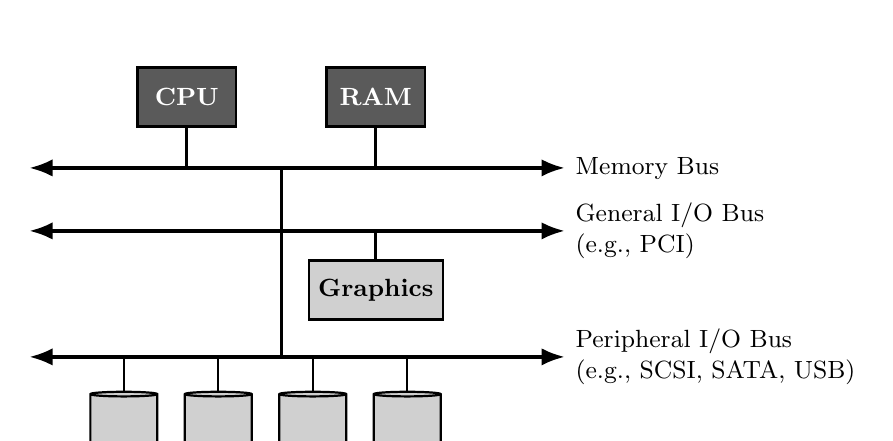
\begin{tikzpicture}[box/.style={draw, thick, minimum width=1.25cm, minimum height=0.75cm, font=\small\bfseries},
                    dsk/.style={cylinder, shape border rotate=90, aspect=0.25, draw, thick, fill=g1,
                                minimum width=0.85cm, minimum height=0.75cm}]
  \node[box, fill=g3, text=white] (cpu) at (2.0,3.9) {CPU};
  \node[box, fill=g3, text=white] (ram) at (4.4,3.9) {RAM};
  \draw[{Latex}-{Latex}, very thick] (0,3.0) -- (6.8,3.0) node[right, font=\small, align=left] {Memory Bus};
  \draw[very thick] (cpu) -- (2.0,3.0);
  \draw[very thick] (ram) -- (4.4,3.0);
  \draw[{Latex}-{Latex}, very thick] (0,2.2) -- (6.8,2.2) node[right, font=\small, align=left] {General I/O Bus\\(e.g., PCI)};
  \draw[{Latex}-{Latex}, very thick] (0,0.6) -- (6.8,0.6) node[right, font=\small, align=left] {Peripheral I/O Bus\\(e.g., SCSI, SATA, USB)};
  \draw[very thick] (3.2,3.0) -- (3.2,0.6);
  \node[box, fill=g1] (gfx) at (4.4,1.45) {Graphics};
  \draw[very thick] (gfx) -- (4.4,2.2);
  \foreach \x in {1.2,2.4,3.6,4.8} {
    \node[dsk] (d\x) at (\x,-0.25) {};
    \draw[thick] (\x,0.6) -- (\x,0.15);
  }
\end{tikzpicture}
\end{center}

\begin{itemize}
  \item The \textbf{CPU} and \textbf{RAM} sit on the fast \textbf{memory bus}.
  \item Fast devices such as \textbf{graphics} hang off a \textbf{general I/O
        bus} (e.g., PCI).
  \item Slow devices such as \textbf{disks} sit on a \textbf{peripheral I/O
        bus} (e.g., SCSI, SATA, USB).
\end{itemize}

\keepspace{8\baselineskip}
\begin{quizbox}[Why use hierarchical buses?]
Physics and cost. The faster a bus is, the \emph{shorter} it must be, so a
high-performance memory bus has little room to plug devices into; and
engineering a bus for high performance is expensive. So the devices that
need high performance (e.g.\ graphics) are placed near the CPU, and many
slower devices share a cheaper, longer bus further away.
\end{quizbox}

\keepspace{14\baselineskip}
% ===========================================================================
\section{The canonical device}
% ===========================================================================

\begin{center}
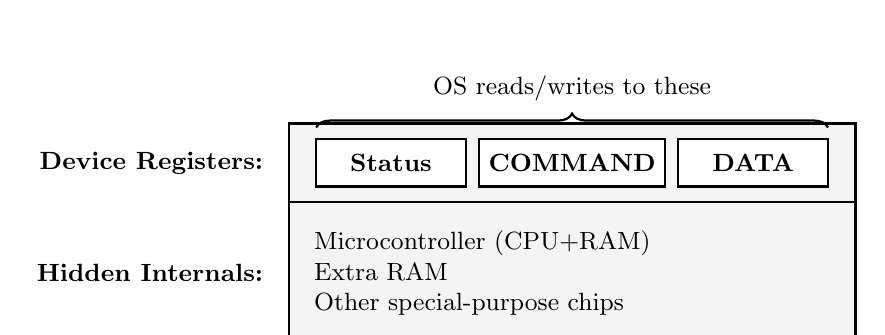
\begin{tikzpicture}[reg/.style={draw, thick, fill=white, minimum width=1.9cm, minimum height=0.6cm, font=\small\bfseries}]
  \draw[thick, fill=boxfill] (0,0) rectangle (7.2,2.8);
  \draw[thick] (0,1.8) -- (7.2,1.8);
  \node[reg] at (1.3,2.3) {Status};
  \node[reg] at (3.6,2.3) {COMMAND};
  \node[reg] at (5.9,2.3) {DATA};
  \node[anchor=west, font=\small, align=left] at (0.2,0.9)
    {Microcontroller (CPU+RAM)\\Extra RAM\\Other special-purpose chips};
  \node[anchor=east, font=\small\bfseries, align=right] at (-0.2,2.3) {Device Registers:};
  \node[anchor=east, font=\small\bfseries, align=right] at (-0.2,0.9) {Hidden Internals:};
  \draw[decorate, decoration={brace, amplitude=5pt}, thick] (0.35,2.75) -- (6.85,2.75)
     node[midway, above=6pt, font=\small] {OS reads/writes to these};
\end{tikzpicture}
\end{center}

A device has two parts:
\begin{itemize}
  \item an \textbf{interface} the OS sees: three \textbf{device registers}.
        The OS reads the \textbf{STATUS} register to see the device's current
        state, writes the \textbf{DATA} register to pass data, and writes the
        \textbf{COMMAND} register to tell the device what to do;
  \item \textbf{hidden internals}: a microcontroller (CPU + RAM), extra RAM,
        and other special-purpose chips that implement the device. The OS
        never sees these.
\end{itemize}

% ===========================================================================
\section{Example write protocol (polling)}
% ===========================================================================

\begin{lstlisting}
while (STATUS == BUSY)   // 1
    ;  // spin
Write data to DATA register          // 2
Write command to COMMAND register    // 3
while (STATUS == BUSY)   // 4
    ;  // spin
\end{lstlisting}

\begin{enumerate}[label=\textbf{\arabic*.}]
  \item Wait until the device is not busy, by repeatedly reading STATUS
        (\textbf{polling}).
  \item Send the data to the DATA register.
  \item Write a command to the COMMAND register; this starts the device.
  \item Wait (polling again) until the device has finished the request.
\end{enumerate}

\subsection{Timeline (built up over the slides)}

Two processes are involved. Process \textbf{A} is running on the CPU, while
the disk is still busy with an earlier request from process \textbf{C}. Now
\textbf{A wants to do I/O}:

\begin{center}
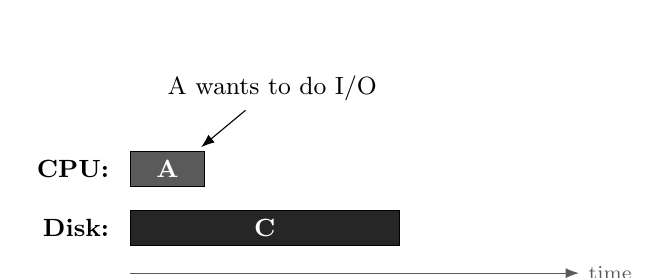
\begin{tikzpicture}[x=0.95cm]
  \rows{6}
  \seg{0.75}{0}{1}{A}{\A}{white}
  \seg{0}{0}{3.6}{C}{\C}{white}
  \node[font=\small, text=black] (w) at (1.9,2.0) {A wants to do I/O};
  \draw[-{Latex}] (w) -- (0.95,1.25);
\end{tikzpicture}
\end{center}

Running the protocol, step by step (each slide highlights the line being
executed):
\begin{enumerate}[label=\textbf{\arabic*.}]
  \item A spins in line 1 while the disk finishes C's request: the CPU is
        busy, but only wasting time.
  \item The disk is free. A copies the data into the DATA register (line 2).
  \item A writes the command (line 3); the disk starts working on A's
        request.
  \item A spins again in line 4 until the disk finishes A's request.
\end{enumerate}
Only then can the CPU run another process, \textbf{B}. (On the slides the
disk's A bar already starts during step 2, while A's data is being moved
onto the device.)

\begin{center}
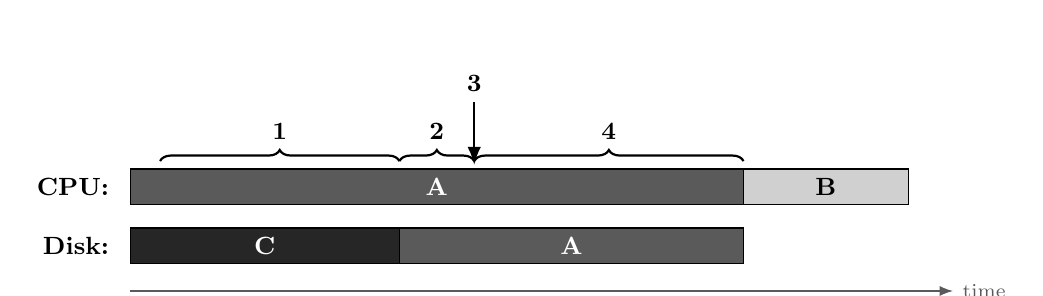
\begin{tikzpicture}[x=0.95cm]
  \rows{11}
  \seg{0.75}{0}{8.2}{A}{\A}{white}
  \seg{0.75}{8.2}{10.4}{B}{\B}{black}
  \seg{0}{0}{3.6}{C}{\C}{white}
  \seg{0}{3.6}{8.2}{A}{\A}{white}
  \draw[decorate, decoration={brace, amplitude=4pt}, thick] (0.4,1.3) -- (3.6,1.3) node[midway, above=4pt, font=\small\bfseries] {1};
  \draw[decorate, decoration={brace, amplitude=4pt}, thick] (3.6,1.3) -- (4.6,1.3) node[midway, above=4pt, font=\small\bfseries] {2};
  \draw[-{Latex}, thick] (4.6,2.05) node[above, font=\small\bfseries] {3} -- (4.6,1.25);
  \draw[decorate, decoration={brace, amplitude=4pt}, thick] (4.6,1.3) -- (8.2,1.3) node[midway, above=4pt, font=\small\bfseries] {4};
\end{tikzpicture}
\end{center}

\begin{warnbox}[How to avoid spinning? Interrupts!]
During steps 1 and 4 the CPU does no useful work. It just keeps reading
STATUS while it could be running B.
\end{warnbox}

% ===========================================================================
\section{Interrupts}
% ===========================================================================

Instead of spinning, the process \textbf{sleeps} and the OS runs someone
else. When the device finishes, it raises a hardware \textbf{interrupt}; the
OS's interrupt handler wakes the waiting process.

\begin{lstlisting}
while (STATUS == BUSY)   // 1
        wait for interrupt;
Write data to DATA register          // 2
Write command to COMMAND register    // 3
while (STATUS == BUSY)   // 4
        wait for interrupt;
\end{lstlisting}

\begin{center}
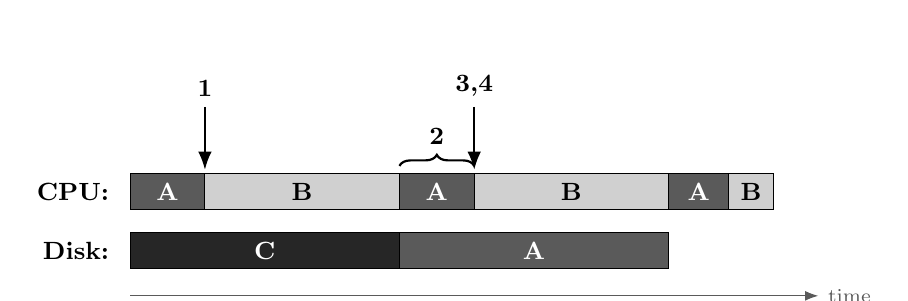
\begin{tikzpicture}[x=0.95cm]
  \rows{9.2}
  \seg{0.75}{0}{1}{A}{\A}{white}
  \seg{0.75}{1}{3.6}{B}{\B}{black}
  \seg{0.75}{3.6}{4.6}{A}{\A}{white}
  \seg{0.75}{4.6}{7.2}{B}{\B}{black}
  \seg{0.75}{7.2}{8}{A}{\A}{white}
  \seg{0.75}{8}{8.6}{B}{\B}{black}
  \seg{0}{0}{3.6}{C}{\C}{white}
  \seg{0}{3.6}{7.2}{A}{\A}{white}
  \draw[-{Latex}, thick] (1,2.05) node[above, font=\small\bfseries] {1} -- (1,1.25);
  \draw[decorate, decoration={brace, amplitude=4pt}, thick] (3.6,1.3) -- (4.6,1.3) node[midway, above=4pt, font=\small\bfseries] {2};
  \draw[-{Latex}, thick] (4.6,2.05) node[above, font=\small\bfseries] {3,4} -- (4.6,1.25);
\end{tikzpicture}
\end{center}

\begin{enumerate}[label=\textbf{\arabic*.}]
  \item A finds the disk busy (with C) and \textbf{sleeps}; the CPU runs B.
  \item The disk finishes C and interrupts; A is woken and copies its data
        into DATA (line 2).
  \item[\textbf{3,4.}] A writes the command and immediately sleeps again; B runs
        while the disk works on A's request. When the disk finishes, it
        interrupts, and A runs again.
\end{enumerate}
The CPU and the disk are now \textbf{overlapped}: both are doing useful work
at the same time.

\keepspace{17\baselineskip}
\subsection{Interrupts vs.\ polling}

\begin{quizbox}[Are interrupts ever worse than polling?]
\begin{itemize}
  \item \textbf{Fast device:} better to spin than to take the interrupt
        overhead. If the device finishes almost immediately, a context switch
        plus an interrupt costs more than a short poll.
  \item \textbf{Device time unknown?} Hybrid approach: spin for a while,
        then use interrupts.
  \item \textbf{Flood of interrupts arrive} (e.g.\ a network card under heavy
        load):
    \begin{itemize}
      \item can lead to \textbf{livelock}: the CPU is always handling
            interrupts and never runs the user processes that would consume
            the work;
      \item better to ignore interrupts while making some progress handling
            them (e.g.\ switch to polling for a while).
    \end{itemize}
  \item \textbf{Other improvement: interrupt coalescing.} Batch together
        several interrupts: the device waits a little before interrupting,
        so one interrupt reports several completions. This lowers the
        overhead, at the cost of some extra delay per request.
\end{itemize}
\end{quizbox}

% ===========================================================================
\section{Protocol variants}
% ===========================================================================

The simple protocol has three parts, and each one has two possible designs:

\begin{center}
\renewcommand{\arraystretch}{1.25}
\begin{tabular}{@{}lll@{}}
  \toprule
  \textbf{Part of the protocol} & \textbf{Option 1} & \textbf{Option 2} \\
  \midrule
  \textbf{Status checks} & polling & interrupts \\
  \textbf{Data} & PIO & DMA \\
  \textbf{Control} & special instructions & memory-mapped I/O \\
  \bottomrule
\end{tabular}
\end{center}

The slides come back to this list three times, each time after one row has
been covered. Status checks were covered above; the next two sections
cover the other two rows.

% ===========================================================================
\section{Data: programmed I/O vs.\ direct memory access}
% ===========================================================================

\begin{quizbox}[What else can we optimize? Data transfer!]
In the interrupt timeline, A's step 2 (copying data into the DATA register)
still uses the CPU. For a large transfer this copying takes a long time,
and the CPU does nothing else during it.
\end{quizbox}

\begin{defbox}[PIO vs.\ DMA]
\textbf{PIO (Programmed I/O):} the CPU directly tells the device what the
data is (the CPU itself moves each word into the device).

\textbf{DMA (Direct Memory Access):} the CPU leaves the data in memory; the
device (a DMA engine) reads the data directly from memory. The CPU still
programs the DMA engine (memory address, length and direction); the engine
then does the copy and interrupts when done.
\end{defbox}

\keepspace{9\baselineskip}
With DMA, line 2 disappears from the CPU's work:

\begin{lstlisting}[escapechar=@]
while (STATUS == BUSY)   // 1
        wait for interrupt;
@\strike{\ttfamily\small Write data to DATA register~~~~~~~~~~// 2}@
Write command to COMMAND register    // 3
while (STATUS == BUSY)   // 4
        wait for interrupt;
\end{lstlisting}

\begin{center}
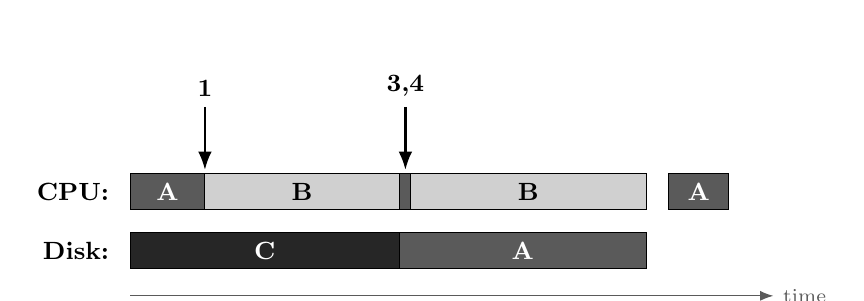
\begin{tikzpicture}[x=0.95cm]
  \rows{8.6}
  \seg{0.75}{0}{1}{A}{\A}{white}
  \seg{0.75}{1}{3.6}{B}{\B}{black}
  \seg{0.75}{3.6}{3.75}{}{\A}{white}
  \seg{0.75}{3.75}{6.9}{B}{\B}{black}
  \seg{0.75}{7.2}{8}{A}{\A}{white}
  \seg{0}{0}{3.6}{C}{\C}{white}
  \seg{0}{3.6}{6.9}{A}{\A}{white}
  \draw[-{Latex}, thick] (1,2.05) node[above, font=\small\bfseries] {1} -- (1,1.25);
  \draw[-{Latex}, thick] (3.68,2.05) node[above, font=\small\bfseries] {3,4} -- (3.68,1.25);
\end{tikzpicture}
\end{center}

A's middle burst shrinks to a thin sliver: it only writes the command and
sleeps. B gets the CPU back sooner, and the disk starts A's request
sooner.

% ===========================================================================
\section{Control: special instructions vs.\ memory-mapped I/O}
% ===========================================================================

\begin{quizbox}[How does the OS read and write registers?]
The protocol reads \textbf{STATUS} (lines 1 and 4) and writes
\textbf{COMMAND} (line 3). How does the CPU actually reach these device
registers?
\end{quizbox}

\begin{center}
\renewcommand{\arraystretch}{1.25}
\begin{tabularx}{\textwidth}{@{}XX@{}}
  \toprule
  \textbf{Special instructions} & \textbf{Memory-mapped I/O} \\
  \midrule
  Each device has a \textbf{port}. & H/W maps the device registers into the
  \textbf{address space}. \\
  \texttt{in}/\texttt{out} instructions (x86) communicate with the device.
  These are privileged, so only the OS can use them. & Ordinary
  \textbf{loads/stores} to those addresses are sent to the device instead of
  to main memory. \\
  \bottomrule
\end{tabularx}
\end{center}

\textbf{Doesn't matter much (both are used).}

% ===========================================================================
\section{Device drivers}
% ===========================================================================

\begin{warnbox}[Variety is a challenge]
\textbf{Problem:} many, many devices, and each has its own protocol.

How can we avoid writing a slightly different OS for each H/W combination?
\end{warnbox}

\begin{keybox}[Solution: write a device driver for each device]
A \textbf{device driver} is the piece of OS code that knows the details of
one device's protocol. The rest of the OS talks to all devices of a kind
through a common interface, and the driver translates.

Drivers are \textbf{70\% of Linux source code}.
\end{keybox}

\subsection{Organization}

\begin{center}
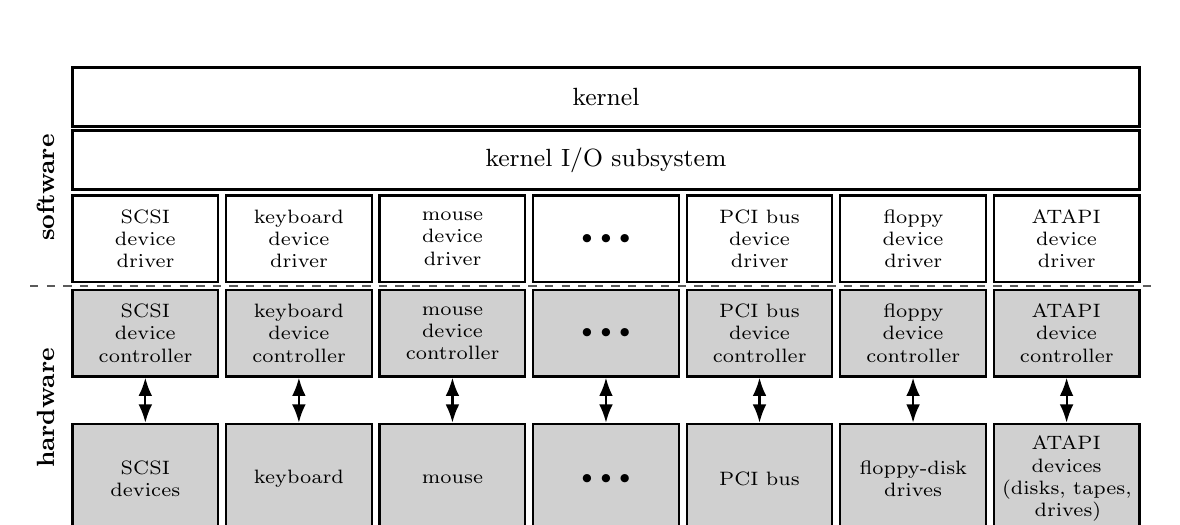
\begin{tikzpicture}[x=1.95cm, y=1cm,
    cell/.style={draw, thick, minimum width=1.85cm, minimum height=1.1cm, align=center, font=\scriptsize, inner sep=1pt, text width=1.75cm}]
  \node[draw, thick, minimum width=13.55cm, minimum height=0.75cm, font=\small] at (3,4.55) {kernel};
  \node[draw, thick, minimum width=13.55cm, minimum height=0.75cm, font=\small] at (3,3.75) {kernel I/O subsystem};
  \foreach \i/\d/\c/\h in {0/SCSI/SCSI/SCSI\\devices, 1/keyboard/keyboard/keyboard, 2/mouse/mouse/mouse,
                           3/$\bullet\bullet\bullet$/$\bullet\bullet\bullet$/$\bullet\bullet\bullet$,
                           4/PCI bus/PCI bus/PCI bus, 5/floppy/floppy/floppy-disk\\drives,
                           6/ATAPI/ATAPI/{ATAPI devices\\(disks, tapes,\\drives)}} {
    \ifnum\i=3
      \node[cell] at (\i,2.75) {\d};
      \node[cell, fill=g1] (c\i) at (\i,1.55) {\c};
    \else
      \node[cell] at (\i,2.75) {\d\\device\\driver};
      \node[cell, fill=g1] (c\i) at (\i,1.55) {\c\\device\\controller};
    \fi
    \node[cell, fill=g1, minimum height=1.4cm] (h\i) at (\i,-0.3) {\h};
    \draw[{Latex}-{Latex}, thick] (c\i.south) -- (h\i.north);
  }
  \node[rotate=90, font=\small\bfseries] at (-0.65,3.4) {software};
  \node[rotate=90, font=\small\bfseries] at (-0.65,0.6) {hardware};
  \draw[dashed, g3, thick] (-0.75,2.15) -- (6.55,2.15);
\end{tikzpicture}
\end{center}

The kernel and the \textbf{kernel I/O subsystem} are common to all devices.
Below them is one \textbf{device driver} per kind of device (software); each
driver talks to its \textbf{device controller} (hardware), which controls
the actual devices.

\subsection{Storage stack}

\begin{center}
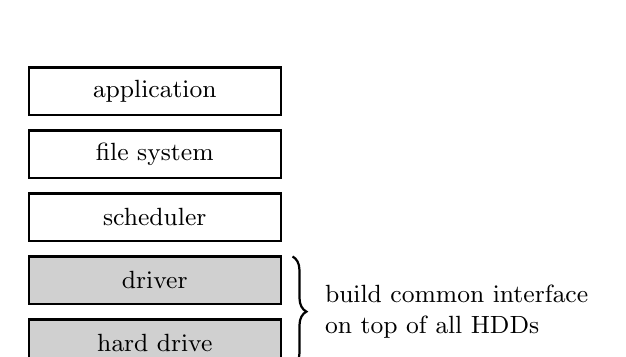
\begin{tikzpicture}[lay/.style={draw, thick, minimum width=3.2cm, minimum height=0.6cm, font=\small}]
  \node[lay] (a) at (0,3.2) {application};
  \node[lay] (f) at (0,2.4) {file system};
  \node[lay] (s) at (0,1.6) {scheduler};
  \node[lay, fill=g1] (d) at (0,0.8) {driver};
  \node[lay, fill=g1] (h) at (0,0) {hard drive};
  \draw[decorate, decoration={brace, amplitude=5pt}, thick] (1.75,1.1) -- (1.75,-0.3)
     node[midway, right=8pt, font=\small, align=left] {build common interface\\on top of all HDDs};
\end{tikzpicture}
\end{center}

The driver hides the details of each particular hard drive, so the layers
above (the I/O scheduler, the file system, the application) work with
\emph{any} disk through one common interface.

% ===========================================================================
\section{Hard disks}
% ===========================================================================

\subsection{Basic interface}

\begin{itemize}
  \item The disk has a \textbf{sector-addressable address space}: it appears
        as an \textbf{array of sectors}.
  \item Sectors are typically \textbf{512 bytes} or 4096 bytes.
  \item Main operations: \textbf{reads + writes to sectors}.
  \item The mechanical (slow) nature makes management ``interesting''.
\end{itemize}

\subsection{Disk internals}

The slides build up the parts of a disk one at a time.

\begin{itemize}
  \item \textbf{Platter:} a circular disk; it is covered with a
        \textbf{magnetic film} that stores the bits.
  \item \textbf{Spindle:} the axle at the centre that the platter is bound to
        and spins around.
  \item \textbf{Surface:} each platter has two surfaces (top and bottom),
        and both can store data.
  \item Many platters may be bound to the spindle.
  \item Each surface is divided into rings called \textbf{tracks}. A
        \textbf{cylinder} is the set of tracks at the same position on every
        surface (across all platters).
  \item The tracks are divided into numbered \textbf{sectors}.
  \item \textbf{Heads} on a moving \textbf{arm} can read from each surface
        (one head per surface, all moved together by the arm).
  \item The spindle/platters rapidly \textbf{spin}.
\end{itemize}

\begin{center}
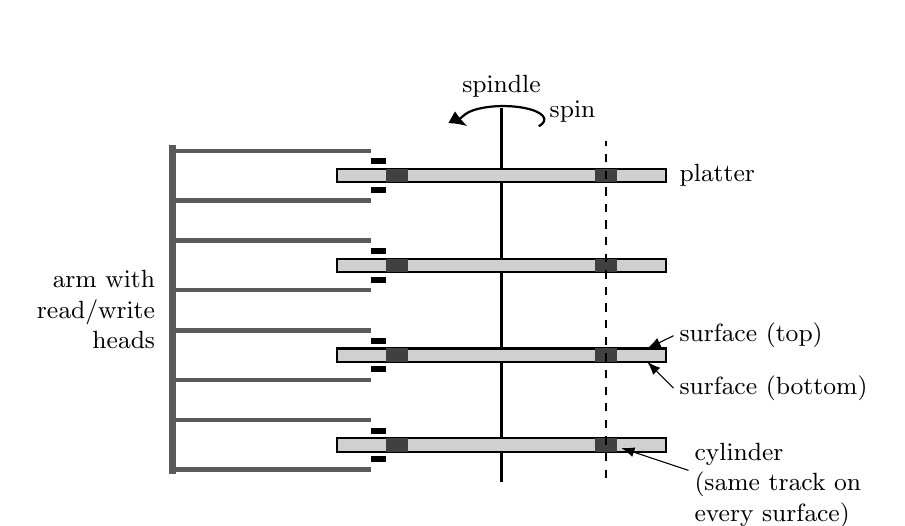
\begin{tikzpicture}[scale=0.95]
  % side view: four platters on a spindle
  \draw[very thick] (0,-0.4) -- (0,4.6);
  \node[above, font=\small] at (0,4.6) {spindle};
  \foreach \y/\c in {0/g1, 1.2/g1, 2.4/g1, 3.6/g1} {
    \fill[\c] (-2.2,\y) rectangle (2.2,{\y+0.18});
    \draw[thick] (-2.2,\y) rectangle (2.2,{\y+0.18});
  }
  % cylinder: same track on every surface
  \foreach \y in {0,1.2,2.4,3.6} {
    \fill[black!75] (1.25,\y) rectangle (1.55,{\y+0.18});
    \fill[black!75] (-1.55,\y) rectangle (-1.25,{\y+0.18});
  }
  \draw[dashed, thick] (1.4,-0.35) -- (1.4,4.15);
  \node[right, font=\small, align=left] at (2.45,-0.45) {cylinder\\(same track on\\every surface)};
  \draw[-{Latex}] (2.5,-0.25) -- (1.6,0.05);
  % arm with heads
  \foreach \y in {0,1.2,2.4,3.6} {
    \draw[line width=1.6pt, g3] (-4.4,{\y+0.42}) -- (-1.75,{\y+0.42});
    \fill[black] (-1.75,{\y+0.32}) rectangle (-1.55,{\y+0.24});
    \draw[line width=1.6pt, g3] (-4.4,{\y-0.24}) -- (-1.75,{\y-0.24});
    \fill[black] (-1.75,{\y-0.14}) rectangle (-1.55,{\y-0.06});
  }
  \draw[line width=2.4pt, g3] (-4.4,-0.3) -- (-4.4,4.1);
  \node[left, font=\small, align=right] at (-4.5,1.9) {arm with\\read/write\\heads};
  \node[right, font=\small] at (2.25,3.7) {platter};
  \node[right, font=\small] at (2.25,1.55) {surface (top)};
  \draw[-{Latex}] (2.3,1.55) -- (1.95,1.38);
  \node[right, font=\small] at (2.25,0.85) {surface (bottom)};
  \draw[-{Latex}] (2.3,0.85) -- (1.95,1.2);
  \draw[-{Latex}, thick] (0.5,4.35) arc[start angle=-30, end angle=210, x radius=0.55, y radius=0.18];
  \node[font=\small] at (0.95,4.55) {spin};
\end{tikzpicture}
\hspace{1.2em}
\begin{tabular}[b]{@{}c@{}}
\tikz{\draw[-{Latex}, thick] (60:1.1) arc[start angle=60, end angle=120, radius=1.1]; \node[font=\small] at (0,1.35) {spin};}\\[-0.6em]
\platter{0}{1.78}{190}{1}
\end{tabular}
\end{center}

\noindent{\small Left: side view (four platters, eight surfaces, one head per
surface; the dark marks are one track on each surface, which together form
a cylinder). Right: top view of one surface as drawn on the slides: three
tracks of 8 sectors, numbered 0--7 (inner), 8--15 (middle), 16--23 (outer),
clockwise from 12 o'clock; sector 12 is highlighted for the example below.}

\keepspace{16\baselineskip}
\subsection{Disk terminology}

\begin{center}
\renewcommand{\arraystretch}{1.18}
\begin{tabularx}{\textwidth}{@{}lX@{}}
  \toprule
  \textbf{Term} & \textbf{Meaning} \\
  \midrule
  spindle & axle at the centre; all platters are bound to it and spin with it \\
  platter & circular disk covered with a magnetic film \\
  surface & one side of a platter (each platter has two) \\
  track & one ring on a surface \\
  cylinder & the stack of tracks at the same position across all platters/surfaces \\
  sector & a numbered piece of a track; the unit the disk reads/writes (512 B or 4 KB) \\
  read/write head & reads/writes one surface; all heads are on one moving arm \\
  \bottomrule
\end{tabularx}
\end{center}

\noindent\textbf{Hard drive demo:}
\begin{itemize}
  \item \url{http://youtu.be/9eMWG3fwiEU?t=30s}
  \item \url{https://www.youtube.com/watch?v=L0nbo1VOF4M}
\end{itemize}

\keepspace{24\baselineskip}
% ===========================================================================
\section{Reading a sector: ``Let's read 12!''}
% ===========================================================================

The head starts over the \textbf{outer} track. Sector 12 is on the
\textbf{middle} track. The slides animate the read in steps:

\begin{center}
\begin{minipage}{\textwidth}\centering
\begin{minipage}[t]{0.3\textwidth}\centering
\platter{0}{1.78}{190}{1}\\[-0.3em]
{\small (a) Let's read 12!\\head on outer track}
\end{minipage}\hfill
\begin{minipage}[t]{0.3\textwidth}\centering
\platter{9}{1.73}{190}{1}\\[-0.3em]
{\small (b) Seek to right track\\(arm moves inward)}
\end{minipage}\hfill
\begin{minipage}[t]{0.3\textwidth}\centering
\platter{56}{1.33}{214}{1}\\[-0.3em]
{\small (c) Wait for rotation\ldots}
\end{minipage}

\medskip
\begin{minipage}[t]{0.3\textwidth}\centering
\platter{275}{1.33}{214}{1}\\[-0.3em]
{\small (d) \ldots wait for rotation}
\end{minipage}\hfill
\begin{minipage}[t]{0.3\textwidth}\centering
\platter{335}{1.33}{214}{1}\\[-0.3em]
{\small (e) Transfer data\\(12 passes under head)}
\end{minipage}\hfill
\begin{minipage}[t]{0.3\textwidth}\centering
\platter{345}{1.33}{214}{1}\\[-0.3em]
{\small (f) Yay! 12 has been read}
\end{minipage}
\end{minipage}
\end{center}

\begin{enumerate}[label=\textbf{\arabic*.}]
  \item \textbf{Seek} to the right track: the arm moves the head from the
        outer track to the middle track.
  \item \textbf{Wait for rotation:} the platter keeps spinning until sector
        12 comes under the head. Here 12 has just gone past the head, so the
        disk must turn most of a full revolution.
  \item \textbf{Transfer data} while sector 12 passes under the head.
        \textbf{Yay!}
\end{enumerate}

\subsection{Positioning}

\begin{itemize}
  \item The drive's \textbf{servo system} keeps the head on track.
  \item How does the disk head know where it is?
    \begin{itemize}
      \item Platters are not perfectly aligned, and tracks are not perfectly
            concentric (\textbf{runout}), so it is difficult to stay on track.
      \item This gets more difficult as the density of disks increases: more
            bits per inch (\textbf{BPI}), more tracks per inch (\textbf{TPI}).
    \end{itemize}
  \item Use a \textbf{servo burst}:
    \begin{itemize}
      \item record placement information every few (3--5) sectors;
      \item when the head crosses a servo burst, figure out the location and
            adjust as needed.
    \end{itemize}
\end{itemize}

\keepspace{12\baselineskip}
% ===========================================================================
\section{Time to read/write}
% ===========================================================================

\begin{keybox}[Three components]
\[
  \text{Time} \;=\; \text{seek} \;+\; \text{rotation} \;+\; \text{transfer time}
\]
\end{keybox}

\subsection{Seek}

\begin{itemize}
  \item Seek cost is a function of \textbf{cylinder distance}, but it is
        \textbf{not a purely linear cost}: the arm must
        \textbf{accelerate, coast, decelerate, settle}.
  \item Settling alone can take \textbf{0.5--2 ms}.
  \item Entire seeks often take several milliseconds: \textbf{4--10 ms}.
  \item Approximate \textbf{average seek distance} \(=\) \textbf{1/3 max seek
        distance} (why?).
\end{itemize}

\keepspace{14\baselineskip}
\begin{solbox}[Why is the average seek distance 1/3 of the maximum?]
This is a continuous approximation: treat the start and target positions
\(x,y\) as uniform on \([0,N]\). The seek distance is \(|x-y|\). Divide the
double integral by the area \(N^2\):
\[
  \int_0^N |x-y|\,dy
  = \int_0^x (x-y)\,dy + \int_x^N (y-x)\,dy
  = x^2 - Nx + \tfrac12 N^2,
\]
\[
  \int_0^N \Bigl(x^2 - Nx + \tfrac12 N^2\Bigr)dx
  = \tfrac13 N^3 - \tfrac12 N^3 + \tfrac12 N^3 = \tfrac{N^3}{3}.
\]
Dividing by \(N^2\) gives an average of \(N/3\): \textbf{one third} of the full
seek distance.
\end{solbox}

\subsection{Rotate}

\begin{itemize}
  \item Depends on rotations per minute (\textbf{RPM}).
  \item \textbf{7200 RPM} is common; \textbf{15000 RPM} is high end.
\end{itemize}

\begin{quizbox}[With 7200 RPM, how long to rotate around?]
\[
  \frac{1}{7200\ \text{RPM}}
  = \frac{1\ \text{minute}}{7200\ \text{rotations}}
  = \frac{1\ \text{second}}{120\ \text{rotations}}
  = 8.3\ \text{ms / rotation}.
\]
\textbf{Average rotation?} On average the target sector is half a turn away:
\(8.3\ \text{ms} / 2 = 4.15\ \text{ms}\).
\end{quizbox}

\subsection{Transfer}

\begin{itemize}
  \item Pretty fast: it depends on RPM and sector density.
  \item \textbf{100+ MB/s} is typical for the maximum transfer rate.
\end{itemize}

\begin{quizbox}[How long to transfer 512 bytes?]
\[
  512\ \text{bytes} \times \frac{1\ \text{s}}{100\ \text{MB}} \approx 5\ \mu\text{s}.
\]
\end{quizbox}

\keepspace{10\baselineskip}
% ===========================================================================
\section{Workload performance}
% ===========================================================================

So\ldots
\begin{itemize}
  \item \textbf{seeks are slow} (milliseconds),
  \item \textbf{rotations are slow} (milliseconds),
  \item \textbf{transfers are fast} (microseconds per sector).
\end{itemize}

\keepspace{11\baselineskip}
\begin{quizbox}[What kind of workload is fastest for disks?]
\begin{itemize}
  \item \textbf{Sequential:} access sectors in order. After one seek and
        rotation, consecutive sectors simply stream under the head, so time
        is \textbf{transfer dominated} (fast).
  \item \textbf{Random:} access sectors arbitrarily. Each request pays its
        own seek and rotation (several ms) to transfer a few \(\mu\)s of
        data, so time is \textbf{seek + rotation dominated} (slow).
\end{itemize}
\end{quizbox}

\keepspace{20\baselineskip}
% ===========================================================================
\section{Summary}
% ===========================================================================

\begin{keybox}[I/O devices and disks]
\begin{itemize}
  \item Buses are hierarchical: CPU and memory on the memory bus, fast
        devices on a general I/O bus (PCI), slow devices on a peripheral bus
        (SCSI, SATA, USB).
  \item A canonical device exposes \textbf{STATUS}, \textbf{COMMAND} and
        \textbf{DATA} registers; its internals are hidden.
  \item Protocol: wait until not busy \(\to\) write data \(\to\) write
        command \(\to\) wait until done. Its variants:
    \begin{itemize}
      \item status checks: \textbf{polling} (wastes CPU) vs.\
            \textbf{interrupts} (overlap CPU and I/O; but bad for fast devices
            and interrupt floods; hybrid and coalescing help);
      \item data: \textbf{PIO} (CPU copies) vs.\ \textbf{DMA} (device reads
            memory itself);
      \item control: \textbf{special in/out instructions} (ports) vs.\
            \textbf{memory-mapped I/O} (loads/stores); both are used.
    \end{itemize}
  \item \textbf{Device drivers} hide device-specific protocols behind a
        common interface; they are 70\% of Linux source code.
  \item A disk is an array of sectors (512 B or 4 KB) on tracks of platter
        surfaces; tracks at the same position form a cylinder; heads on one
        arm; platters spin.
  \item \(\text{Time} = \text{seek} + \text{rotation} + \text{transfer}\).
        Seek is 4--10 ms (average distance \(=\) 1/3 of max); rotation at 7200
        RPM is 8.3 ms per turn (4.15 ms average); transfer is about 5
        \(\mu\)s per 512 B at 100 MB/s.
  \item Sequential workloads are transfer dominated (fast); random workloads
        are seek + rotation dominated (slow).
\end{itemize}
\end{keybox}

\end{document}
